% BHU PYQ -- Manually transcribed & corrected
% Paper: MTB-604 : Discrete Mathematics
% Exam: B.A./B.Sc. (Hons.) Semester VI Examination, 2022-23

\documentclass[11pt,a4paper]{article}
\usepackage[a4paper,top=2.5cm,bottom=2.5cm,left=2.8cm,right=2.8cm,headheight=14pt]{geometry}
\usepackage{amsmath,amssymb}
\usepackage[T1]{fontenc}
\usepackage[utf8]{inputenc}
\usepackage{lmodern}
\usepackage{microtype}
\usepackage{fancyhdr}
\usepackage{enumitem}
\usepackage{hyperref}
\usepackage{lastpage}
\usepackage{parskip}
\usepackage{tikz}

\hypersetup{colorlinks=true,urlcolor=black,linkcolor=black,
  pdftitle={MTB-604: Discrete Mathematics -- BHU PYQ},pdfauthor={Banaras Hindu University}}

\pagestyle{fancy}
\fancyhf{}
\renewcommand{\headrulewidth}{0.4pt}
\renewcommand{\footrulewidth}{0.4pt}
\fancyhead[L]{\small   \textit{Banaras Hindu University}}
\fancyhead[R]{\small   \textit{MTB-604: Discrete Mathematics}}
\fancyfoot[C]{\small Page  \thepage\ of \pageref{LastPage}}


\newlist{parts}{enumerate}{2}
\setlist[parts,1]{label=(\alph*),leftmargin=*,itemsep=5pt,topsep=3pt}
\setlist[parts,2]{label=(\roman*),leftmargin=*,itemsep=3pt,topsep=2pt}

\newcommand{\pts}[1]{\hfill   \textit{[#1]}}


\begin{document}


\begin{center}
  {\large\bfseries BANARAS HINDU UNIVERSITY}\\[2pt]
  {
\normalsize B.A./B.Sc. (Hons.) Semester VI Examination, 2022-23}\\[6pt]
  \rule{0.8\linewidth}{0.5pt}\\[6pt]
  {\large\bfseries Paper No. MTB-604: Discrete Mathematics}\\[4pt]
  {
\normalsize Time: 3 Hours\hfill Maximum Marks: 70}
\end{center}

\rule{\linewidth}{0.4pt}

\smallskip



\noindent   \textit{Instructions: Answer   \textbf{five} questions including Question~1 which is compulsory. Symbols have their usual meanings.}

\bigskip




\noindent   \textbf{Question 1.}   \textit{(Compulsory --- 2 marks each.)}

\begin{parts}
  \item Construct the truth table of the logical expression:
  \[ (p \lor q) \land 
eg(p \land q) \]
  \item Rewrite the following statements without using the conditional operator ($\rightarrow$):
  
\begin{parts}
    \item If it is cold, he wears a hat.
    \item If productivity increases, then wages rise.
  \end{parts}
  \item How many reflexive relations are there on a set with $n$ elements?
  \item What is a totally ordered set (chain)? Present an example of a poset which is not totally ordered, and justify your answer.
  \item Let $(L, \le)$ be a lattice. If $a \le b$, then prove that for any $c \in L$:
  \[ a \land c \le b \land c \]
  \item Draw all possible trees with exactly 5 vertices.
  \item What is an Euler circuit? Find an Eulerian path for the following graph, if it exists:
  
\begin{center}
    
\begin{tikzpicture}[node distance=1.8cm, every node/.style={circle, draw, fill=black!10, minimum size=18pt, inner sep=0pt}]
      
ode (A) {$A$};
      
ode (B) [right of=A] {$B$};
      
ode (C) [right of=B] {$C$};
      
ode (D) [below of=A] {$D$};
      
ode (E) [below of=B] {$E$};
      
ode (F) [below of=C] {$F$};
      
      \draw (A) -- (B);
      \draw (B) -- (C);
      \draw (A) -- (D);
      \draw (B) -- (E);
      \draw (C) -- (F);
      \draw (D) -- (E);
      \draw (E) -- (F);
      \draw (A) -- (E);
      \draw (E) -- (C);
    \end{tikzpicture}
  \end{center}
\end{parts}

\medskip\rule{\linewidth}{0.2pt}

\medskip


\noindent   \textbf{Question 2.}

\begin{parts}
  \item Let $p$ be ``It is cold'' and let $q$ be ``It is raining''. Give a simple verbal sentence which describes each of the following statements: \pts{6}
  
\begin{parts}
    \item $
eg p$
    \item $p \land q$
    \item $p \lor q$
    \item $q \lor 
eg p$
    \item $p \rightarrow q$
    \item $p \leftrightarrow q$
  \end{parts}
  \item Show that $
eg(p \lor q) \lor (
eg p \land q)$ and $
eg p$ are logically equivalent by developing a series of logical equivalences. \pts{4}
  \item When is a compound statement called: (i) a tautology, (ii) a contradiction, and (iii) a contingency? Give a simple example for each case. \pts{4}
\end{parts}

\medskip\rule{\linewidth}{0.2pt}

\medskip


\noindent   \textbf{Question 3.}

\begin{parts}
  \item Consider the conditional proposition $p \rightarrow q$. State its converse, inverse, and contrapositive propositions. Which of these propositions, if any, are logically equivalent to $p \rightarrow q$? Justify your answers. \pts{6}
  \item Negate each of the following statements: \pts{4}
  
\begin{parts}
    \item All students live in the dormitories.
    \item Some students are 25 years old or older.
  \end{parts}
  \item Prove that if $n$ is an integer and $3n+2$ is odd, then $n$ is odd. \pts{4}
\end{parts}

\medskip\rule{\linewidth}{0.2pt}

\medskip


\noindent   \textbf{Question 4.}

\begin{parts}
  \item Define a lattice. What are the distributive laws of a lattice? Give an example of a lattice in which the distributive laws (i) hold, and (ii) do not hold. Justify your answer. \pts{6}
  \item Draw the Hasse diagram representing the partial order relation $R = \{(a, b) \mid a  \text{ divides } b\}$ on the set $S = \{2, 4, 5, 10, 12, 20, 25\}$. Find the maximal and minimal elements. \pts{4}
  \item Determine the poset whose Hasse diagram is given below. Is this poset a lattice? Justify your answer. \pts{4}
  
\begin{center}
    
\begin{tikzpicture}[node distance=1.5cm, every node/.style={circle, draw, fill=black!10, minimum size=15pt, inner sep=0pt}]
      
ode (base) {$a$};
      
ode (x) [above left of=base] {$b$};
      
ode (y) [above right of=base] {$c$};
      
ode (top) [above right of=x] {$d$};
      
      \draw (base) -- (x);
      \draw (base) -- (y);
      \draw (x) -- (top);
      \draw (y) -- (top);
    \end{tikzpicture}
  \end{center}
\end{parts}

\medskip\rule{\linewidth}{0.2pt}

\medskip


\noindent   \textbf{Question 5.}

\begin{parts}
  \item Obtain the complete Conjunctive Normal Form (CNF) and Disjunctive Normal Form (DNF) of the Boolean function:
  \[ f(x, y, z, w) = xy + xzw \] \pts{6}
  \item Use a Karnaugh map to find a minimal sum-of-products (SOP) form for the Boolean expression:
  \[ F(x, y, z, t) = xy't + xyzt + x'y'z' + x'yzt' \]
  Moreover, draw the logic circuit corresponding to that minimal Boolean expression. \pts{6+2}
\end{parts}

\medskip\rule{\linewidth}{0.2pt}

\medskip


\noindent   \textbf{Question 6.}

\begin{parts}
  \item Let $G$ be a connected planar simple graph with $e$ edges and $v$ vertices. Let $r$ be the number of regions in a planar representation of $G$. Prove that:
  \[ r = e - v + 2 \] \pts{6}
  \item Prove or disprove that the complete graph $K_5$ and the complete bipartite graph $K_{3,3}$ are non-planar. \pts{4}
  \item When are two graphs said to be isomorphic? Determine, with justification, whether the following two graphs $G_1$ and $G_2$ are isomorphic: \pts{4}
  
\begin{center}
    
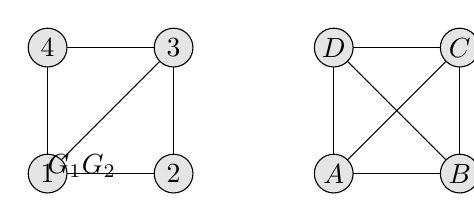
\begin{tikzpicture}[scale=0.8, every node/.style={circle, draw, fill=black!10, minimum size=14pt, inner sep=0pt}]
      \draw (0,0) node (1) {$1$}
         -- (2,0) node (2) {$2$}
         -- (2,2) node (3) {$3$}
         -- (0,2) node (4) {$4$}
         -- cycle;
      \draw (1) -- (3);
      
ode at (1,-0.7) {$G_1$};
      
      \draw (4,0) node (A) {$A$}
         -- (6,0) node (B) {$B$}
         -- (6,2) node (C) {$C$}
         -- (4,2) node (D) {$D$}
         -- cycle;
      \draw (A) -- (C);
      \draw (B) -- (D);
      
ode at (5,-0.7) {$G_2$};
    \end{tikzpicture}
  \end{center}
\end{parts}

\medskip\rule{\linewidth}{0.2pt}

\medskip


\noindent   \textbf{Question 7.}

\begin{parts}
  \item Let $G$ be the following undirected weighted graph:
  
\begin{center}
    
\begin{tikzpicture}[scale=0.9, auto, every node/.style={circle, draw, fill=black!10, minimum size=16pt, inner sep=0pt}]
      
ode (a) at (0,1.5) {$a$};
      
ode (b) at (2,3) {$b$};
      
ode (c) at (2,0) {$c$};
      
ode (d) at (4,3) {$d$};
      
ode (e) at (4,0) {$e$};
      
ode (f) at (6,1.5) {$f$};
      
ode (g) at (8,1.5) {$g$};
      
      \path (a) edge node [above left] {3} (b)
            (a) edge node [below left] {4} (c)
            (b) edge node [above] {2} (d)
            (b) edge node [right] {3} (c)
            (c) edge node [below] {5} (e)
            (d) edge node [right] {1} (e)
            (d) edge node [above right] {4} (f)
            (e) edge node [below right] {2} (f)
            (f) edge node [above] {3} (g);
    \end{tikzpicture}
  \end{center}
  
\begin{parts}
    \item Use Kruskal's algorithm to find a Minimum Spanning Tree (MST) of $G$. \pts{5}
    \item Use Dijkstra's shortest path algorithm to compute the shortest path from source vertex $a$ to the destination vertex $g$ of the graph $G$. \pts{5}
  \end{parts}
  \item Prove that any tree with at least two vertices has at least two pendant (leaf) vertices. \pts{4}
\end{parts}

\vfill
\rule{\linewidth}{0.4pt}

\begin{center}\small
\href{https://bhu-exam.vercel.app/}{Click here to visit our website}\\[4pt]
\href{https://me-aryan.vercel.app/}{Click here to visit our contributor}\\[4pt]
\href{https://quashan-me.vercel.app/}{Click here to visit our contributor}
\end{center}

\end{document}
